\chapter{Event Reconstruction and Linearity}
\label{Linearity}
% Uniformity Study 
% New Event recon 
% Linearity Software 

\section{Introduction}
Following the results of the uniformity study, the event reconstruction was revisited to establish how we can improve the quality of the projection data. The event reconstruction makes use of both \acrshort{COM} and \acrshort{ML} reconstruction algorithms. We discussed the advantages of the \acrshort{LRF} correction in \acrshort{ML} here we outline how the reconstruction implemented corrections for instability. 

\section{Event Reconstruction}
The event reconstruction is initialised with the \acrshort{COM} reconstruction, making use of a minimum count baseline to remove scatter events. This initial reconstruction is used by the \acrshort{ML} algorithm to establish a final projection image. Producing the \acrshort{LRF} models take a long time and so we proposed a normalised \acrshort{LRF} approach for more adaptable modelling. The list-mode data were normalised with respect to the mean counts in order to reduce the effect of anomalous events. The \acrshort{LRF} and \acrshort{COM} projections were then produced using the normalised list mode data. This ensured they matched and would account for hot spots or faulty channels in the data. The normalised \acrshort{LRF} could now be applied to any acquisition as instability corrections can be included without reproducing a new model.
\paragraph{}
The existing event reconstruction software required manual energy window selection. To reduce processing time, this was replaced with an automatic process which made use of a peak finding algorithm and defined window width. However, it was found that events outside of the \acrshort{UFOV} would reduce the performance of the peak finding algorithm as high scatter peaks were present in the energy spectra. A filter mask was introduced in the peak finder to remove the events outside the \acrshort{UFOV}, the energy window would be calculated from the remaining events. The event reconstruction would reconstruct all events with this window, not just the \acrshort{UFOV}. Figure \ref{fig:MaskEW} shows how energy spectra are improved by the filter mask. 

\begin{figure}[!t]
%\vspace{-0.2cm}
\centering
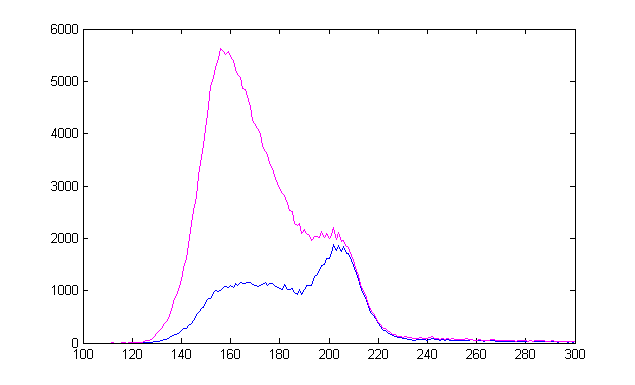
\includegraphics[width=3.6in]{figures/new_spectrum.png}

    \caption{The pink curve shows the unfiltered spectra with a false peak due to scatter. The blue curve shows the true photopeak.} \label{fig:MaskEW}
%\vspace{-0.2cm}
\end{figure}

This reconstruction proved useful when applying corrections and creating linearity correction maps. Hot spots were reduced by the normalised reconstruction resulting in reduced errors when measuring uniformity or linearity. Normalised calibration data is used in the next section in order to improve linearity modelling.

\section{Linearity}
As discussed in chapter \ref{Milan} the experiments showed the need for regular system calibration. The system stability and existing calibration procedures and software proved impractical for clinical use. The presence of truncated data and the need for manual intervention in the software is unreliable and not reproducible. To account for instability and reduce the calibration time we set out to implement an improved calibration and acquisition procedure. A new calibration software was required to implement a new calibration protocol.
\paragraph{}
This new linearity method would mimic the BULMA software by making use of spline models, however, to avoid the truncation issues we approached the linearity correction through a simple geometric transform. We first need to validate the proposed linearity software. To validate the geometric transform method we first implement it on the existing linearity data acquired from the \acrshort{HSR} and \acrshort{UCH} experiments. Three methods of measuring linearity are described here. 

\subsection{Methods}
To carry out the linearity correction we must first take a measure of linearity distortion within each detector and the determine a correction transformation for the distortion. Each of the three methods built a series of spline models which would fit the linearity line data and determine the distortion in each given line. These spline models were then optimised against the linearity data. The method of optimisation was different in each and so we set out to determine the best option. 
\paragraph{}
The first method built a spline model and simulated a linearity data set. To build the spline model a set of control points were defined. The linearity projections present bands of event data. By taking a profile through a sample of the band data  we defined an array of peaks and troughs. The peaks in the array defined the position of each linearity band; by measuring the peak positions of profiles across the whole linearity data we defined a set of control points. A continuous spline was then defined along each control point giving a measure of linearity distortion. The splines were then used to define a discrete model, this was a simulated image of the linearity data with consistent values from 0 to 1. The simulated data is normalised to the linearity data. The spline control points were then optimised using a Levenberg-Marquardt algorithm and a similarity measure of the simulated image against the real data. The optimisation will stop when the spline model matches the linearity data, by a given target tolerance. 
\paragraph{}
The second method optimised the splines by maximising the coverage of the individual splines across the linearity data. The control points and spline models are defined in the same way as the first method. Instead of creating a digitised image, the spline model is used to extract a path across the linearity data. Each spline defines a window of 5 pixels either side of each point in the spline. This window of pixels is integrated and the values are recorded. As the splines need to define the bright bands, we optimise the spline control points to maximise the integral. This spans the spline path across the brightest region which should define the linearity bands. 
\paragraph{}
Both methods required smoothing and noise removal to aid with the optimisation steps; this proved inconsistent and so a non-optimisation method was explored. The previous methods were initialised by finding a few control points along each line of data, using a peak finding algorithm. The third method uses this algorithm to scan across every pixel and find as many control points as possible. This was not possible in the optimisation methods as it would take too long to optimise. The linearity data was first processed to removed noise and underwent a uniformity correction; this helped to highlight the linearity data making the peaks more defined. The resulting spline was found to follow the distortion without further optimisation. 
\paragraph{}
Following each method two spline models were defined: X linearity was defined by 19 splines and Y linearity was defined by 41 splines. Overlaying these models gave 779 crossing points. The known geometry of the linearity collators was used to define a set of 779 fixed positions, each associated to a crossing point. A geometric transform was calculated to map the crossing points to the collimator geometry, using a piece-wise linear transform. The resulting transform would then be applied to all acquisition data.

\subsection{Results}
The first method was able to define the distortion of the linearity data. However, the simulated images proved to be difficult to define. Discrete splines would limit the curvature possible when measuring the distortion, making subtle changes impossible to model. The simulated data presented problems as it could force a match if too many corrections were applied, resulting in a false termination of the optimiser.
\paragraph{}
The integration method proved more accurate for smaller distortions as the spline model remained continuous. However, more control points were required to carry out this method which slowed the optimisation. It was also harder to control the spline paths and so crossing splines were more likely with this method. 
\paragraph{}
The peak finder method was the fastest and most robust method. As it used the most control points, it could define splines in the presence of faulty channels. The fast computational run time allowed it to be repeated easily if the splines failed. 

\subsection{Discussion}
Each method proved capable of producing splines to follow the linearity data. However only the first and last method produced consistent results for practical use. Method 1 was used to define the linearity correction of the data collected in \acrshort{HSR}, this data had few errors and was well defined. However, the method required some manual intervention in order to account for faulty channels or great linear distortion. 
\paragraph{}
The data collected in \acrshort{UCH} was less stable and so method 1 was unable to account for the greater distortion without a lot of manual corrections. For this reason, method 3 was developed and was used to produce the linearity maps for this data. Detector instability meant some manual intervention was required, however as method 3 was fast and robust this was easily done. 
\section{Conclusion}
The results of the uniformity study and production of linearity maps highlighted the importance of quality control during acquisition and event reconstruction. As we continue to carry out experiments we set to monitor the uniformity and stability of the detectors more regularly, so that corrections or repeat measurements can be implemented as required.
\paragraph{}
Normalising the event reconstruction improved the projection data, however, it was unable to correct for stability. The instability of the detectors leads to many repeat measurements which proved time-consuming. The need for a calibration procedure that can be quickly reproduced is essential to carry out the necessary corrections. We can use the linearity software as a starting point for this new calibration procedure. The new methods are more versatile than the BULMA software and can be adapted for use in a new calibration method. Future works set out to implement this procedure. Figures \ref{fig:UncorrLin}, \ref{fig:ParCorrLin} and \ref{fig:CorrLin} show the results of applying the linearity maps to the calibration data. 

\begin{figure}[!tbp]
  \centering
  \subfloat[Uncorrected linearity projection.]{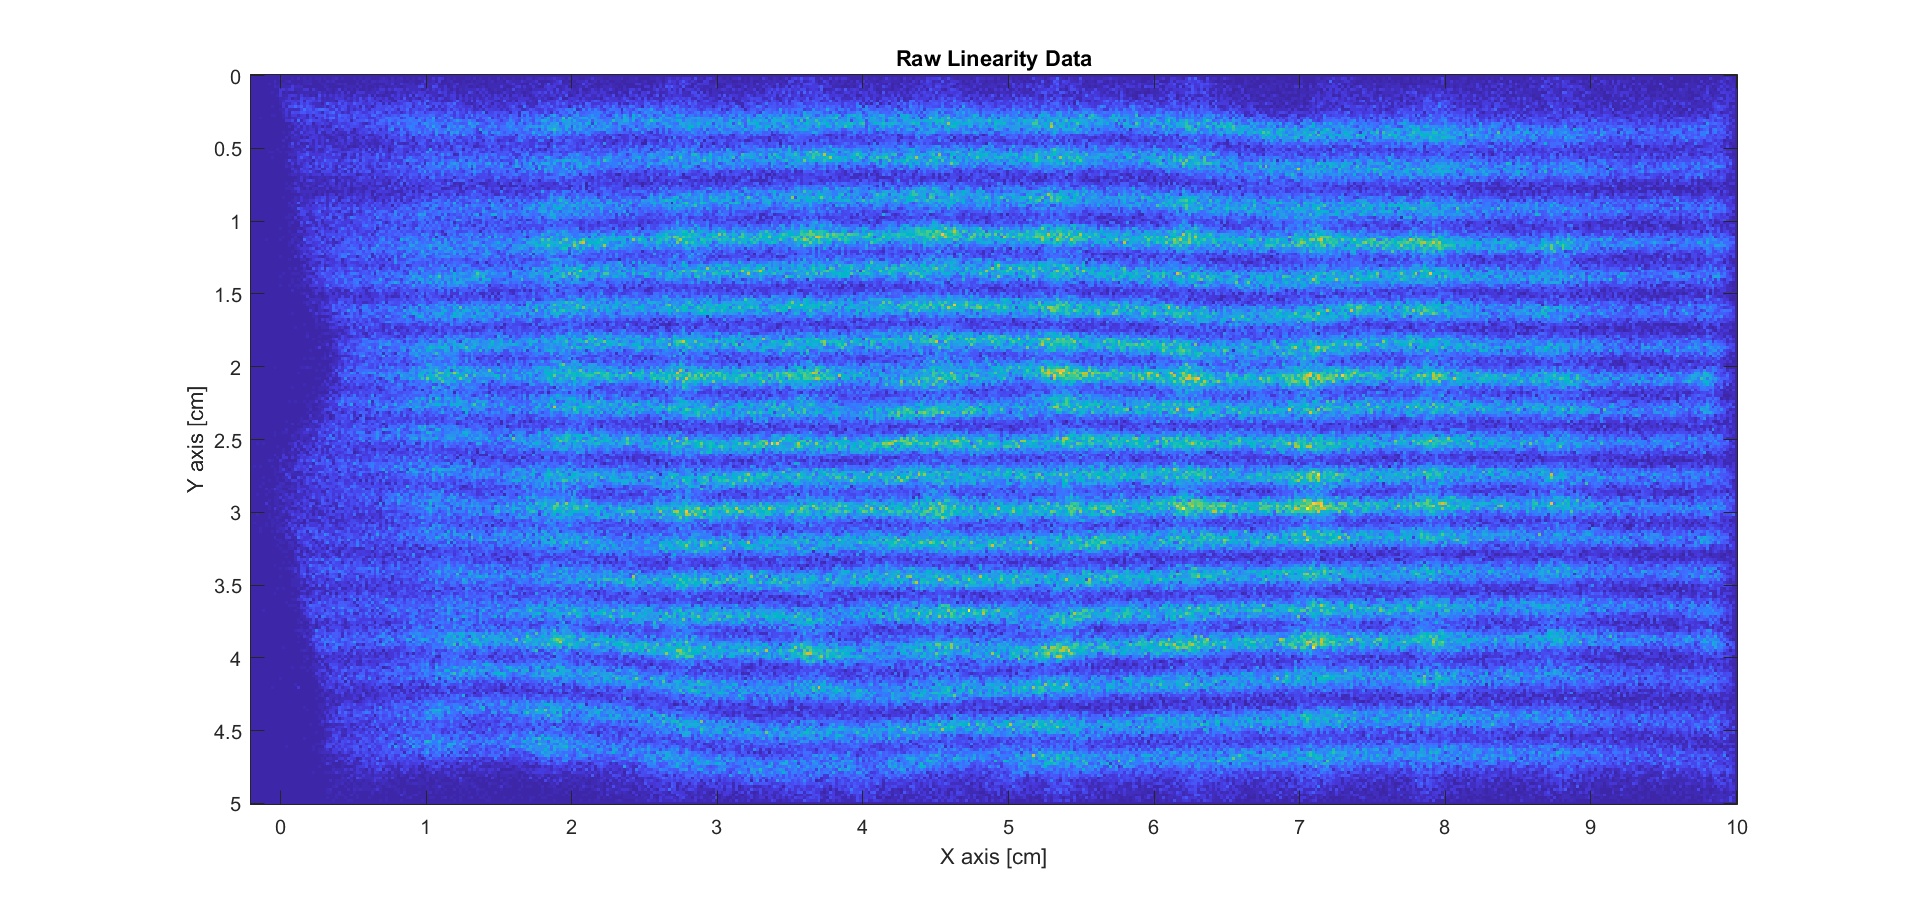
\includegraphics[width=0.8\textwidth]{figures/LinUncorr.png}\label{fig:UncorrLin}}
  \hfill
  \subfloat[Linearity correction applied.]{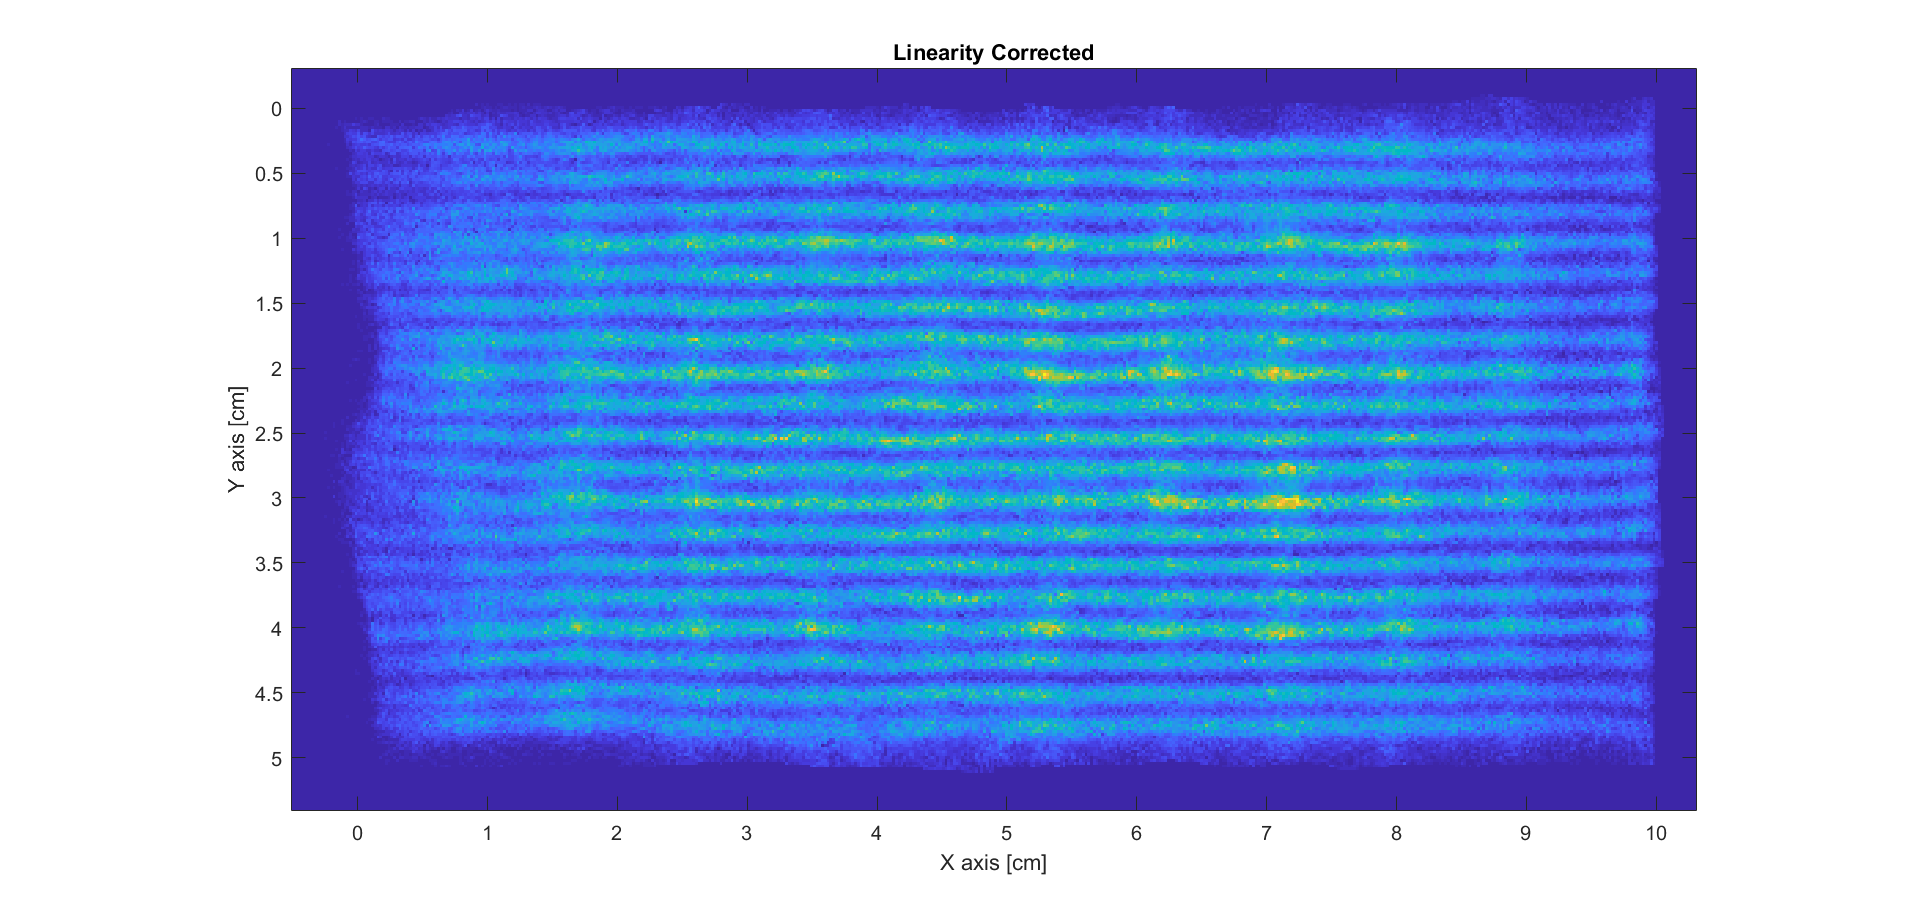
\includegraphics[width=0.8\textwidth]{figures/LinParCorr.png}\label{fig:ParCorrLin}}
    \hfill
  \subfloat[Linearity and Uniformity applied.]{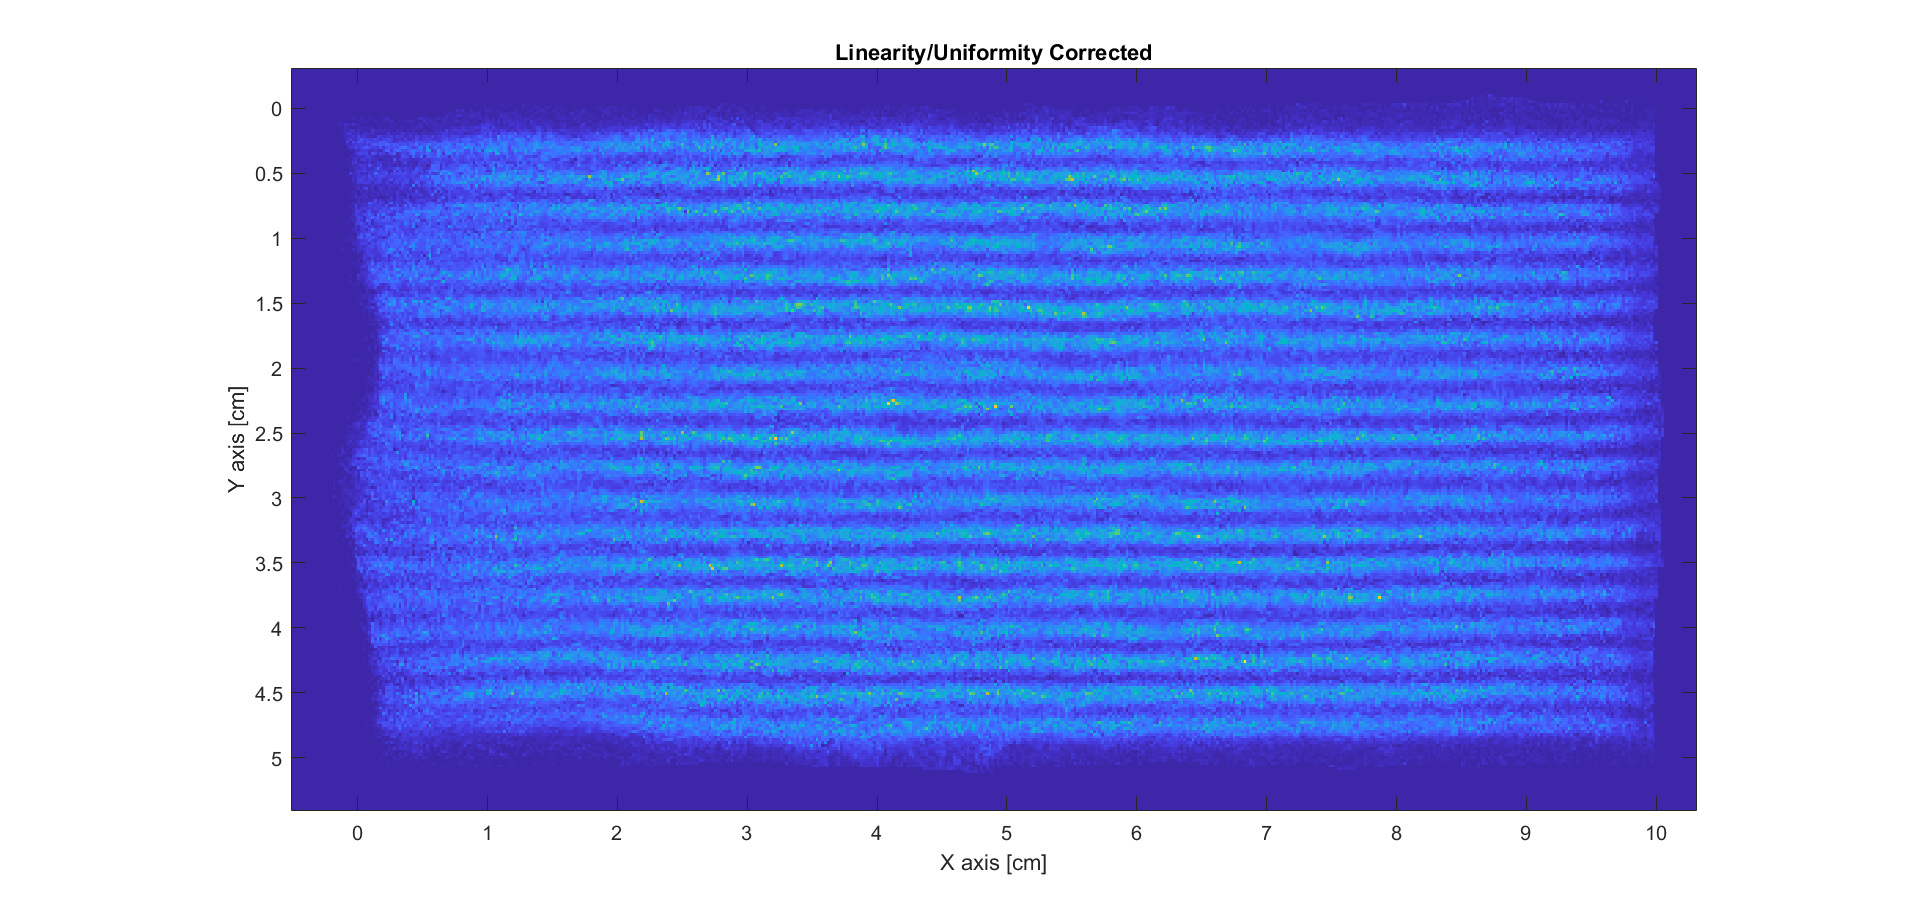
\includegraphics[width=0.8\textwidth]{figures/LinCorr.png}\label{fig:CorrLin}}
  \caption{The linearity data is corrected using the geometric based software producing correct projections.}
\end{figure}
